\documentclass{article}
\usepackage[utf8]{inputenc}
\usepackage{hyperref}
\usepackage{graphicx}
\usepackage{float}

\hypersetup{
    colorlinks=true,
    linkcolor=blue,
    filecolor=magenta,      
    urlcolor=cyan,
    pdftitle={Overleaf Example},
    pdfpagemode=FullScreen,
    }

\title{Vector Visualization}
\author{Caleb Edwards}
\date{January 2022}

\begin{document}

\maketitle

\section*{Introduction}
Most vector data is in 2 or 3D, which means most software represents vector data as 3D with z component as null.
\\\\
An important domain for vector visualization in CFD (computational fluid dynamics). CFD simulations predict time-dependent behavior of compressible 3D fluid flows.

% *************************** SECTION 6.1 *********************************
\section*{6.1 - Divergence and Vorticity}
\subsection*{Divergence}
If v is a 3D vector field that represents a flow field that transports mass, the \textbf{divergence (div)} of v characterizes the gain/loss of mass at a given point p in the vector field in unit time. Divergence of a vector in a scalar. Divergence computes the \href{http://www-solar.mcs.st-and.ac.uk/~alan/MT3601/Fundamentals/node6.html}{flux} (surface integral of a vector field over a closed surface) that the vector field transports through the imaginary boundary. Divergence outputs a scalar field given a vector field. 
\begin{equation}
    \textbf{div v} = \frac{\partial v_x}{\partial x} + \frac{\partial v_y}{\partial y} + \frac{\partial v_z}{\partial z}
\end{equation}
\begin{itemize}
    \item Positive Divergence Points (sources) - spread from points outwards
    \item Negative Divergence Points (sinks) - mass gets sucked into points
    \item Zero Divergence - no spread or suck / no compression or expansion
\end{itemize}

\subsection*{Vorticity}
Given a 3D vector field v, the \textbf{vorticity} of v (curl or rotor of $v^2$) is the vector quantity. Vorticity of a vector is a vector. Vorticity computes the rotation flux around a point. The magnitude of vorticity expresses the speed of angular rotation. The direction of vorticity indicates direction perpendicular to the plane of rotation.

\begin{equation}
    \textbf{rot v} = (\frac{\partial v_z}{\partial y} - \frac{\partial v_y}{\partial z}, \frac{\partial v_x}{\partial z} - \frac{\partial v_z}{\partial x}, \frac{\partial v_y}{\partial x} - \frac{\partial v_x}{\partial y})
\end{equation}
The vorticity vector characterizes the speed and direction of rotation of a given vector field at every point
\\\\
\textbf{Vortex} is a region where the vector field locally circles around a point called the \textbf{vortex center}. High divergence and high vorticity are typically complimentary. Cone shapes seem to be a good example of this. When applying curl and divergence metrics, the div rot v = 0 for any vector field v.
\\\\
\textbf{Turbulent Flows} : high number of vortices and the alternation of their spinning direction (fluid dynamics and aerodynamics). The \textbf{streamwise vorticity} is how quickly v turns itself around.
\begin{equation}
    \Omega = \frac{v \cdot \texttt{rot v}}{||v||}
\end{equation}
\\
\textbf{Helicity} is one half the scalar product of the velocity and vorticity vectors. This represents a corkscrew-like local motion. Used in weather studies for understanding severe convective storms and tornadoes, since in strong updrafts, the velocity and vorticity vectors seem to be aligned, yielding high helicity.
\\\\
We need the \textbf{partial derivatives} of the vector field components. For discrete data, these can be approximated using formulas specific for every grid type (section 3.7).

% *************************** SECTION 6.2 *********************************
\section*{6.2 - Vector Glyphs}
\textbf{Vector Glyphs} are probably the simplest, and fastest, and most popular technique for visualizing vector fields. This involves associating a vector glyph/icon to every sample point of the dataset. Various properties of the icon, such as location, direction, orientation, size, and color are adjusted to reflect the value of the vector attribute it represents.
\\\\
\textbf{Line Glyphs} - Lines show position, direction, and magnitude of a set of vectors. Oriented line glyphs are sometimes called \textbf{hedgehogs}, due to spiky appearance. We can use sub-sampling to make the visualization more readable. Color can also be applied to lines instead of magnitude. Hedgehog clarity depend strongly on the glyph scaling factor.
\\\\
\textbf{Cone and Arrow Glyphs} - These can be used to show a signed direction compared to the lines. They just take more space to draw, which creates more clutter, which means lower resolution datasets.
\\\\
\textbf{Concerns} - cannot be pixel by pixel since glyphs take up multiple pixels, which affects inverse image-to-data mapping. The glyph technique provides a purely discrete visualization which can sometimes be very hard to interpolate what the data is doing. 

For 3D vector glyphs, resolution is a big problem. Subsampling is a good first alleviation. Can also draw the glyphs transparently and in monochrome. We can also take select surfaces in the 3D model and draw those glyphs. 
\\\\
To summarize, this way of visualization is easy to implement and intuitive, but can have problems such as occlusion, subsampling artifacts, and poor visualization.

\begin{figure}[H]
\caption{Tornado contour plot with vector magnitude glyphs at z=0}
\centering
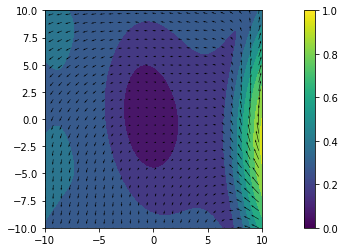
\includegraphics[scale=0.55]{tornado_2d_contour_glyphs.png}
\end{figure}

\begin{figure}[H]
\caption{Tornado contour plot with vector magnitude glyphs at z=64 or midpoint}
\centering
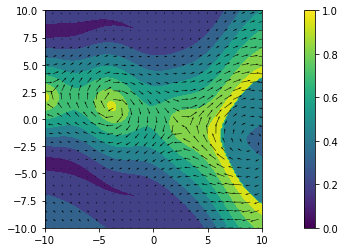
\includegraphics[scale=0.55]{tornado_2d_contour_mid.png}
\end{figure}

\begin{figure}[H]
\caption{Magnitude glyph plot sub-sampled every 50 points }
\centering
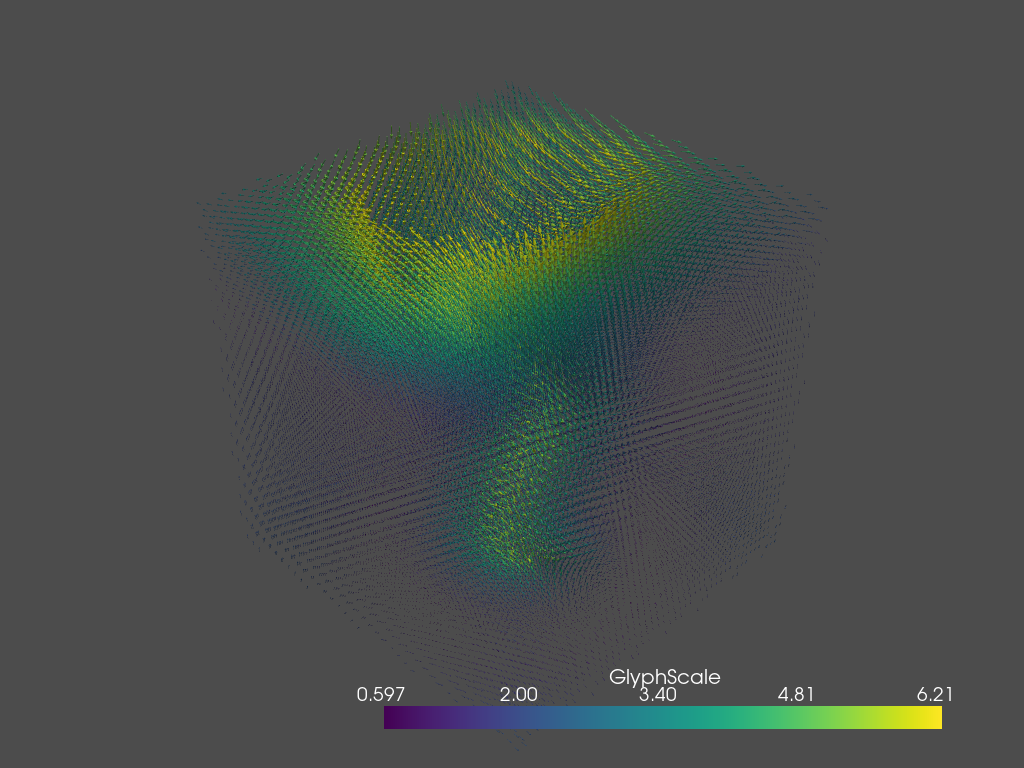
\includegraphics[scale=.4]{tornado_glyph_sample_50.png}
\end{figure}

% *************************** SECTION 6.3 *********************************
\section*{6.3 - Vector Color Coding}
\textbf{Vector Color Coding} - associates a color with every point of a given surface on which we have defined a vector dataset. Usually uses a HSV system for colors or aka a color wheel. Color encodes vector orientation and direction. Vector orientation is encoded in the hue and the vector length is encoded in the value. Extensive training is needed to interpret the inverse mapping from hue to vector orientation, especially when trying to decode 3D.

\begin{figure}[H]
\caption{Tornado vector color coded sampled every 10 points.}
\centering
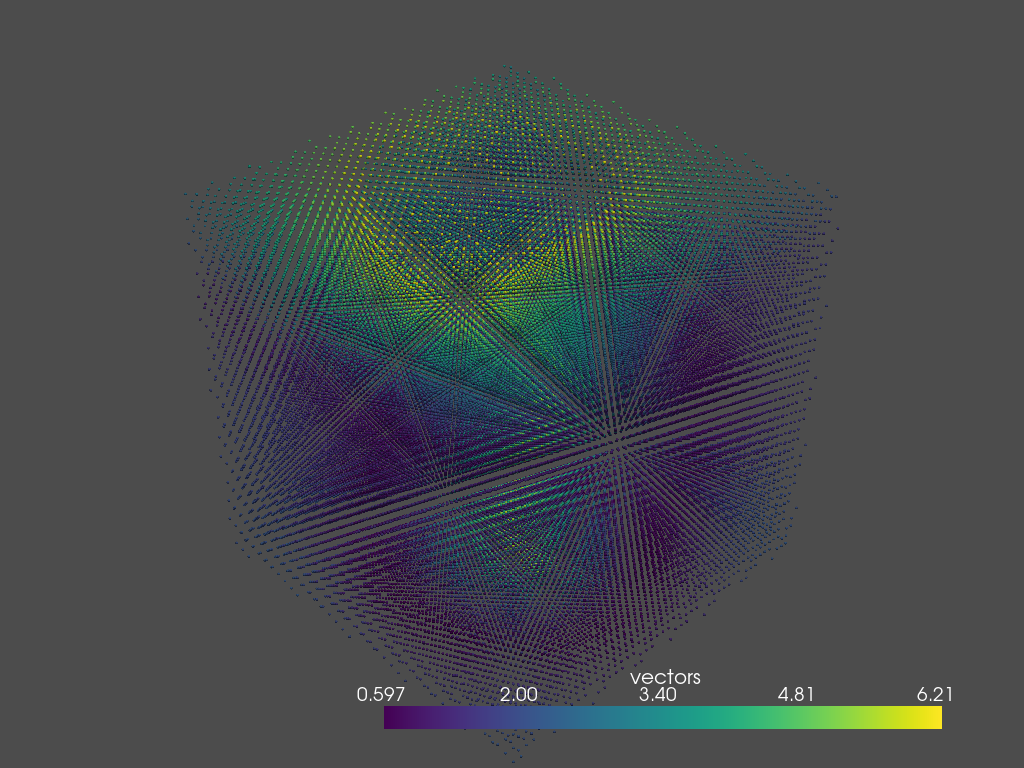
\includegraphics[scale=.4]{tornado_color_coding.png}
\end{figure}

% *************************** SECTION 6.4 *********************************
\section*{6.4 - Displacement Plots}
\textbf{Displacement Plots / Warped Plots} - Instead of displaying trajectories, like the glyph plots, displacement plots show only the endpoint of those trajectories. They produce a continuous result. Still more abstract and harder to visualize than vector glyphs. They are a warped surface in the vector field. The below equation represents a new surface

\begin{equation}
    p'_i = p_i + kv'(p_i)
\end{equation}
\\
v' is a vector field that controls the displacement of the surface S. v' can be set to v, the original vector field. k is the displacement factor that needs to be chosen carefully. Too large k can result in too much warping, which results in self intersecting. Small k results in not warped enough, which provides bad visualization.
\\\\
Two graphs seem to be associated to a 3D vector dataset. Figure 6.12.a shows the flow of the fluid, inlet to outlet. Figure 6.12.b. Shows the motion of the object in the direction perpendicular to its surface.
\\\\
Still harder to interpret than vector glyphs. Figure 6.13 shows an example of a plot that has been overwarped. A warped plot is in Figure 6.12, where the coloring is the warping of the original data. Does not perform well when displacement is along a surface.

% *************************** SECTION 6.5 *********************************
\section*{6.5 - Stream Objects}
\textbf{Stream Objects} are more of a family of techniques, related by the idea of visualizing the trajectory of some input object in a vector field over a given/longer time interval than vector glyphs.

\begin{itemize}
    \item Time-Dependent Vector Fields
    \begin{itemize}
        \item v : D x T
        \item At some spatial position in D, the vector field v(x,t) can have different values for different time moments
        \item \textbf{Pathlines}
        \begin{itemize}
            \item Can use the streamline equation in 6.10 by creating a fixed time
            \item Compute the actual path in a time dependent vector field $\rightarrow \frac{dx(t)}{dt} = v(x(t), t)$
        \end{itemize}
        \item \textbf{Streaklines}
        \begin{itemize}
            \item Take $x_0$ from D and over T assume that fluid is released from $x_0$. This fluid will get advected into the vector field v(x,t) and create a time-dependent curve with the flow.
            \item $\frac{dx(\tau, t)}{dt} = v(x(\tau, t))$
            \item $x(\tau = t, t) = S_{path}(\tau)$
            \item $x(0, 0) = x_0$
        \end{itemize}
    \end{itemize}
     
    \item Time-Independent Vector Fields 
    \begin{itemize}
        \item v : D
        \item The spatial position does not change with time
        \item \textbf{Streamlines} % PAGE 35 in Paraview Tutorial
        \begin{itemize}
            \item A curved path starting from a given point $x_0$ which is tangent at v
            \item $S_{stream}(\tau) = x(\tau) \rightarrow$ where $\tau$ represents the arc-length coordinate along the curve
            \item $\frac{dx(\tau)}{d\tau} * v(x(\tau)) = 0 \rightarrow \frac{dx(\tau)}{d\tau} = v(x(\tau))$
            \item Streamline is a curved path over a given time interval of a trace particle passing through a given start location or seed point
            \item Require numerical integration, which accumulates errors as the integration time increases
        \end{itemize}
    \end{itemize} 
\end{itemize}
\\
Streamlines, pathlines, and streaklines are result in the same curves and provide identical results.
\\\\
% Need to better understand traces
Streamline Calculation - Euler integration (Eq. 6.13). This is the simplest, but least accurate. Since streamline is not discretized and provides curved lines, Euler allows a way to discretize t and replaces the integral with a sum.
\\\\
Runge-Kutta method provides more accuracy by taking two vector points and averaging them to get a more accurate streamline
\\\\
$\Delta t$ is hard to predict, and a compute $\Delta t$ while running the algorithm is best approach to give most accurate results.
\\\\
Coverage of a Streamline - every dataset point should be a small distance away from some streamline. 
\\\\
The density of the streamlines in the final image should have a max and min. Longer streamlines are preferred over short ones.
\\\\
Dense streamline solutions - trace a streamline until it gets close to any other streamline or itself and have an iterative insertion of seed points in undersampled areas. Then can discard too short streamlines and try new seed points until average length is up. Good example of streamlines is in Figure 6.15.
\\\\
\textbf{Stream Tubes} - In addition to plain lines, graphical shapes can be used with the streamlines. For 3D, undersampling is key to make the visualization understandable and less cluttered. A good example of a traced stream tube is in Figure 6.20.
\\\\
\textbf{Stream Ribbons} - Launch two streamlines close to each other. If the two streamlines stay relatively close to each other then the stream ribbon's twisting around its center curve gives a measure of the twisting of the vector field around the direction of advection. % Need to better understand advection
\\\\
\textbf{Stream Surfaces} - two dimensional, so easier to follow visually. Flow described by the vector field is always tangent to the surface. Need to be careful around high divergence. 
\\\\
\textbf{Streak Surfaces} - For time-dependent vector fields, streak surfaces generalize the notion of streak lines the same way stream surfaces generalize the notion of stream lines. Seed curve of a stream tube is a small closed curve, like a circle. For a stream ribbon is is a short line segment. 

% *************************** SECTION 6.6 *********************************
\section*{6.6 - Texture-Based Vector Visualization}
\textbf{ Texture-Based Vector Visualization} provide a way to have \textbf{continuous} visualization representation (piecewise continuous signal). They are used for more dense data compared to the glyph technique. Can use graininess for the encoding of the direction. Can use the line integral convolution principle to find the color of the cells in a grid. Can then have a streamline passing through the grid as in figure 6.24. This process is thought of as blurring the noise image along the streamlines. This is thought of as advecting and injecting noise textures. OpenGL is used for many of these equations in computing the IBFV visualization.
\\\\
\textbf{Image Based Flow Visualization (IBFV)} method is another way to represent texture-based vector visualization. Produces anitmated flow textures in real-time. The advection in time of the property I in a 2D vector field is given by:

\begin{equation}
    I(x+v(x,t)\Delta t, t+\Delta t) = I(x,t)
\end{equation}
\\
This is forward advection, stating the property I at a location downstream at a future moment. To create an animated flow texture to go with this advection property, we need to add an injection-term / dye into the flow domain. 
\\\\
Steps to implement IBFV:
\begin{itemize}
    \item NOISE = 32 Samples (enough to capture periodic behavior)
    \item f = simple step function (others can be used)
    \item Initialization
    \item Endless loop (advection, noise injection, and construction of the work texture)
    \item reference Listing 6.2
\end{itemize}
Figure 6.28b shows a good example of a texture based visualization where ink was advected in the flow field. 
\\\\
LIC (Line Integral Convolution) is a process of blurring or filtering the texture (noise) image along the streamlines. Due to blurring, the pixels along a streamline are getting smoothed; the graininess of texture is gone. However, between neighboring streamlines, the graininess of texture is preserved, showing contrast.

% *************************** SECTION 6.7 *********************************
\section*{6.7 - Simplified Representation of Vector Fields}
Data should not be represented the same in every case. Need to choose the best \textbf{features} of the vector field for the output that you want. Regions that exhibit important characteristic for an application area, should be visualized in different ways compared to the less important ones. Only keep the important features.
\\\\
Classification of 2D critical points for a 2D vector field found in Figure 6.31 determined from Eigenvalues and Eigenvectors.
\\\\
\textbf{Parabolic Sectors} - Streamlines in $S_i$ have one end at c.
\\
\textbf{Elliptic Sectors} - Strealines in $S_i$ have both ends at c.
\\
\textbf{Hyperbolic Sectors} - Strealines in $S_i$ do not pass through c.
\\
\\
\textbf{Field Decomposition Methods}
\begin{enumerate}
    \item This method partitions the vector data into regions of string intraregion and weak interregion similarity. Meanining, separate by strength of intraregion.
    \item Core - find similarity metric that defines how similar two regions are, because this leads to different decompositions depending on how different they are. Compare the direction and magnitude of the vector.
    \item Perform a top-down partitioning or bottom-up agglomerative clustering of dataset
    \item AMG (Algebraic MultiGrid) - The idea of producing a hierarchy of bases that approximates a given vector field at several levels of detail
\end{enumerate}


% *************************** SECTION 6.8 *********************************
\section*{6.8 - Illustrative Vector Field Rendering} % Page 43 in Paraview Tutorial
\textbf{Depth-Dependent Halos} use a set of streamlines represented as curves. Not ribbons because they are oriented parallel towards the viewing plane. Used to visualize 3D vector fields. Only uses two colors.

% *************************** Conclusion *********************************
\section*{Conclusion}
Simple visual representations, straightforward implementation : vector glyph
Multiscale textures animated in real time, complex implementations: LIC
\\\\
\href{https://journals.iucr.org/j/services/editguide.html}{Greek Letters}
\\
\href{https://www.cs.sjtu.edu.cn/~shengbin/course/datavis/LEC6.Vector.Visualization.pdf}{Helpful Slides}
\\
\href{https://ebookcentral-proquest-com.dist.lib.usu.edu/lib/usu/reader.action?docID=1605634&ppg=196}{Book}

% *************************** Paraview *********************************
\section*{Paraview}
\href{https://www.paraview.org/}{Paraview}\\
\href{https://www.paraview.org/Wiki/ParaView_Self-directed_Tutorial}{Paraview Tutorial}\\\\
Use the color map editor to view the datasets with different transparencies
\textbf{Transformations}
\begin{enumerate}
    \item Streamlines
    \begin{enumerate}
        \item stream tracer
        \begin{enumerate}
            \item stream tracer is looking for a vector dataset to perform this operation on - i.e. Tornado : u*iHat + v*jHat+w*kHat
            \item glyph - can add glyphs to stream % page 37
        \end{enumerate}
        \item tube - to make thicker
        \item Compare Properties
        \begin{enumerate}
            \item clip
            \item plot over line % page 39
        \end{enumerate}
    \end{enumerate}
    \item Time
    \begin{enumerate}
        \item Rescale to Data Range - If coloring looks bad % page 53
        \item Temporal Interpolator - Smoothes time lapse video
    \end{enumerate}
\end{enumerate}

% *************************** VTK *********************************
\section*{VTK}
\href{https://kitware.github.io/vtk-examples/site/Python/}{VTK for Python}\\
\href{https://cgl.ethz.ch/research/visualization/data.php}{VTI Datasets}
% Create a visualization in stk for each section and paste picture in each section


\section*{Data Format}
\href{https://docs.pyvista.org/index.html}{pyvista} is a package built on top of vtk that allows interaction with the data through numpy. A \href{https://docs.pyvista.org/user-guide/what-is-a-mesh.html}{mesh} is any spatially referenced information and usually consists of geometrical representations of a surface or volume in 3D space.
\\\\
Points are vertices on the mesh. All pyvista datasets are meshes, and all meshes have points. Most points have connectivity with other points. This is represented as a cell. A cell is defined by the connectivity or topology of the mesh.
\\\\
Attributes are data values that live on the point or cell of a mesh. In the case of the tornado dataset, there is a u,v,w array associated with each point in the dataset. This would be the vector at that point. The attributes at each point in the tornado are u,v,w, which represent the vector at that point.

% Make vector glyphs more visual
% Change the opacity to be a transfer function based on the magnitude

% Plot lines for time data
% particle tracer/lines in paraview

% Add to github repo

\end{document}
